\chapter{Auto-Encoding Variational Bayes}
\label{ch:vae}

\section{Descriptive Overview: The Latent Variable Paradigm}

Deep learning has traditionally excelled at mapping inputs to outputs via deterministic transformations. However, to genuinely understand a data generating distribution---to synthesize novel examples, perform interpolation, or discover underlying causal factors---we must cast our neural networks as directed probabilistic models. The Auto-Encoding Variational Bayes (AEVB) framework provides a mathematically rigorous method to train directed generative models containing continuous latent variables. 

At its core, AEVB fuses two traditionally distinct domains: variational inference from Bayesian statistics and auto-encoder architectures from deep learning. The fundamental challenge it addresses is the intractability of posterior inference. In a generative model where a complex data point $x \in \mathcal{X}$ (such as an image) is generated from a set of lower-dimensional latent factors $z$, evaluating the true posterior distribution $p_\theta(z|x)$ is generally intractable if the likelihood is parameterized by a non-linear neural network. The integral required to compute the marginal likelihood (or evidence) cannot be analytically evaluated, nor easily approximated.

Before AEVB, the dominant approach to dealing with intractable posteriors involved Markov Chain Monte Carlo (MCMC) methods. While theoretically sound, MCMC methods are often prohibitively slow, struggling to mix in high dimensions and failing to scale to modern deep learning datasets $\mathcal{D}$. Variational inference approaches this problem differently: rather than sampling, we reframe inference as an optimization problem. We posit a family of tractable approximate posteriors and find the member of this family that is closest to the true posterior in terms of Kullback-Leibler divergence. 

The breakthrough of AEVB lies in \textit{amortized} inference. Instead of solving a separate optimization problem for the latent variables of each data point, AEVB employs an \textit{inference network} (the encoder) that learns a direct mapping from the data space to the parameters of the approximate posterior. The generative process (the decoder) and the inference process (the encoder) are parameterized by neural networks and trained jointly. They optimize a single, unified objective function known as the Evidence Lower Bound (ELBO). This framework not only makes deep generative modeling computationally feasible but also provides a profound information-theoretic perspective on representation learning: the model must compress the data into a latent representation $z$ while preserving enough information to decode the original signal.

\section{The Mathematical Core}

\subsection{Derivation of the Evidence Lower Bound}
Let $\mathcal{D} = \{x_1, \dots, x_N\}$ be a dataset consisting of $N$ i.i.d.\ samples of a variable $x$. We assume the data is generated by a random process involving an unobserved continuous random variable $z$. The generative model is given by the joint distribution $p_\theta(x, z) = p_\theta(x|z) p_\theta(z)$, where $p_\theta(z)$ is a prior distribution over the latent variables, and $p_\theta(x|z)$ is the decoder likelihood parameterized by $\theta$.

The marginal likelihood of a single datapoint is:
\begin{equation}
    p_\theta(x) = \int p_\theta(x|z) p_\theta(z) dz
\end{equation}
For a highly non-linear $p_\theta(x|z)$, this integral is intractable. Consequently, the true posterior $p_\theta(z|x) = p_\theta(x|z)p_\theta(z) / p_\theta(x)$ is also intractable. We introduce an inference model $q_\phi(z|x)$, the encoder parameterized by $\phi$, to approximate it.

\begin{theorem}[The Evidence Lower Bound]
\label{thm:elbo}
For any valid approximate posterior $q_\phi(z|x)$, the log marginal likelihood is bounded below by the Evidence Lower Bound (ELBO), denoted as $\mathcal{L}(\theta, \phi; x)$:
\begin{equation}
    \log p_\theta(x) \ge \mathcal{L}(\theta, \phi; x) = \mathbb{E}_{q_\phi(z|x)}[\log p_\theta(x|z)] - D_{\text{KL}}(q_\phi(z|x) \parallel p_\theta(z))
\end{equation}
\end{theorem}

\begin{proof}
We begin by expressing the log marginal likelihood $\log p_\theta(x)$ as an expectation over $q_\phi(z|x)$, and apply Bayes' theorem:
\begin{align}
    \log p_\theta(x) &= \mathbb{E}_{q_\phi(z|x)}[\log p_\theta(x)] \\
    &= \mathbb{E}_{q_\phi(z|x)}\left[\log \frac{p_\theta(x, z)}{p_\theta(z|x)}\right] \\
    &= \mathbb{E}_{q_\phi(z|x)}\left[\log \left( \frac{p_\theta(x, z)}{q_\phi(z|x)} \frac{q_\phi(z|x)}{p_\theta(z|x)} \right)\right] \\
    &= \mathbb{E}_{q_\phi(z|x)}\left[\log \frac{p_\theta(x, z)}{q_\phi(z|x)}\right] + \mathbb{E}_{q_\phi(z|x)}\left[\log \frac{q_\phi(z|x)}{p_\theta(z|x)}\right] \\
    &= \mathcal{L}(\theta, \phi; x) + D_{\text{KL}}(q_\phi(z|x) \parallel p_\theta(z|x))
\end{align}
Because the Kullback-Leibler divergence is non-negative ($D_{\text{KL}} \ge 0$), it strictly follows that:
\begin{equation}
    \log p_\theta(x) \ge \mathcal{L}(\theta, \phi; x)
\end{equation}
Expanding the first term yields the final form of the ELBO:
\begin{align}
    \mathcal{L}(\theta, \phi; x) &= \mathbb{E}_{q_\phi(z|x)}\left[\log \frac{p_\theta(x|z) p_\theta(z)}{q_\phi(z|x)}\right] \\
    &= \mathbb{E}_{q_\phi(z|x)}[\log p_\theta(x|z)] - D_{\text{KL}}(q_\phi(z|x) \parallel p_\theta(z))
\end{align}
\end{proof}

\begin{figure}[htbp]
    \centering
    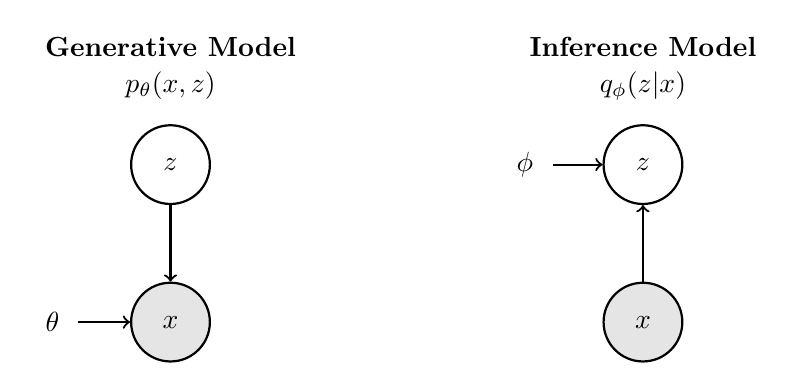
\begin{tikzpicture}[
        obs/.style={circle, draw, fill=gray!20, minimum size=1cm, thick},
        latent/.style={circle, draw, fill=white, minimum size=1cm, thick},
        param/.style={circle, draw=none, minimum size=0.5cm},
        arrow/.style={->, thick}
    ]
    % Generative Model
    \node[latent] (z_gen) at (0,0) {$z$};
    \node[obs] (x_gen) at (0,-2) {$x$};
    \node[param] (theta) at (-1.5,-2) {$\theta$};
    \draw[arrow] (z_gen) -- (x_gen);
    \draw[arrow] (theta) -- (x_gen);
    \node at (0, 1.5) {\textbf{Generative Model}};
    \node at (0, 1) {$p_\theta(x, z)$};
    
    % Inference Model
    \node[obs] (x_inf) at (6,-2) {$x$};
    \node[latent] (z_inf) at (6,0) {$z$};
    \node[param] (phi) at (4.5,0) {$\phi$};
    \draw[arrow] (x_inf) -- (z_inf);
    \draw[arrow] (phi) -- (z_inf);
    \node at (6, 1.5) {\textbf{Inference Model}};
    \node at (6, 1) {$q_\phi(z|x)$};
    \end{tikzpicture}
    \caption{Directed graphical models corresponding to the decoder (left) and the encoder (right).}
    \label{fig:graphical_model}
\end{figure}

The objective in AEVB is to maximize $\mathcal{L}(\theta, \phi; x)$ with respect to both $\theta$ and $\phi$. The $\mathbb{E}_{q_\phi(z|x)}[\log p_\theta(x|z)]$ term represents a reconstruction log-likelihood. The $D_{\text{KL}}(q_\phi(z|x) \parallel p_\theta(z))$ term acts as a complexity penalty, bounding the information rate required to encode $x$ into the latent representation $z$. 

\subsection{The Reparameterization Trick}
While optimizing $\theta$ via Monte Carlo sampling is trivial, optimizing the inference parameters $\phi$ is exceedingly difficult because the expectation is taken with respect to the distribution $q_\phi(z|x)$ itself. Using the standard REINFORCE algorithm yields gradients with prohibitively high variance. AEVB elegantly resolves this by deterministically reparameterizing the random variable $z$.

\begin{theorem}[The Reparameterization Trick]
\label{thm:reparam}
Let $z$ be a continuous random variable distributed according to $q_\phi(z|x)$. Suppose there exists a differentiable, deterministic transformation $g_\phi(x, \epsilon)$ and an independent base distribution $p(\epsilon)$ such that if $\epsilon \sim p(\epsilon)$, then $g_\phi(x, \epsilon) \sim q_\phi(z|x)$. The gradient of an expectation of a function $f(z)$ can be exactly expressed as:
\begin{equation}
    \nabla_\phi \mathbb{E}_{q_\phi(z|x)}[f(z)] = \mathbb{E}_{p(\epsilon)}[\nabla_\phi f(g_\phi(x, \epsilon))]
\end{equation}
\end{theorem}
\begin{proof}
By the Law of the Unconscious Statistician (LOTUS), we rewrite the expectation over $z$ as an expectation over the base noise variable $\epsilon$:
\begin{align}
    \nabla_\phi \mathbb{E}_{q_\phi(z|x)}[f(z)] &= \nabla_\phi \int q_\phi(z|x) f(z) dz \\
    &= \nabla_\phi \int p(\epsilon) f(g_\phi(x, \epsilon)) d\epsilon \\
    &= \int p(\epsilon) \nabla_\phi f(g_\phi(x, \epsilon)) d\epsilon \\
    &= \mathbb{E}_{p(\epsilon)}[\nabla_\phi f(g_\phi(x, \epsilon))]
\end{align}
Assuming standard regulatory conditions to exchange the gradient and the integral (such as dominated convergence), the gradient operator moves safely inside the expectation, allowing low-variance Monte Carlo estimation via deterministic backpropagation.
\end{proof}

\begin{figure}[htbp]
    \centering
    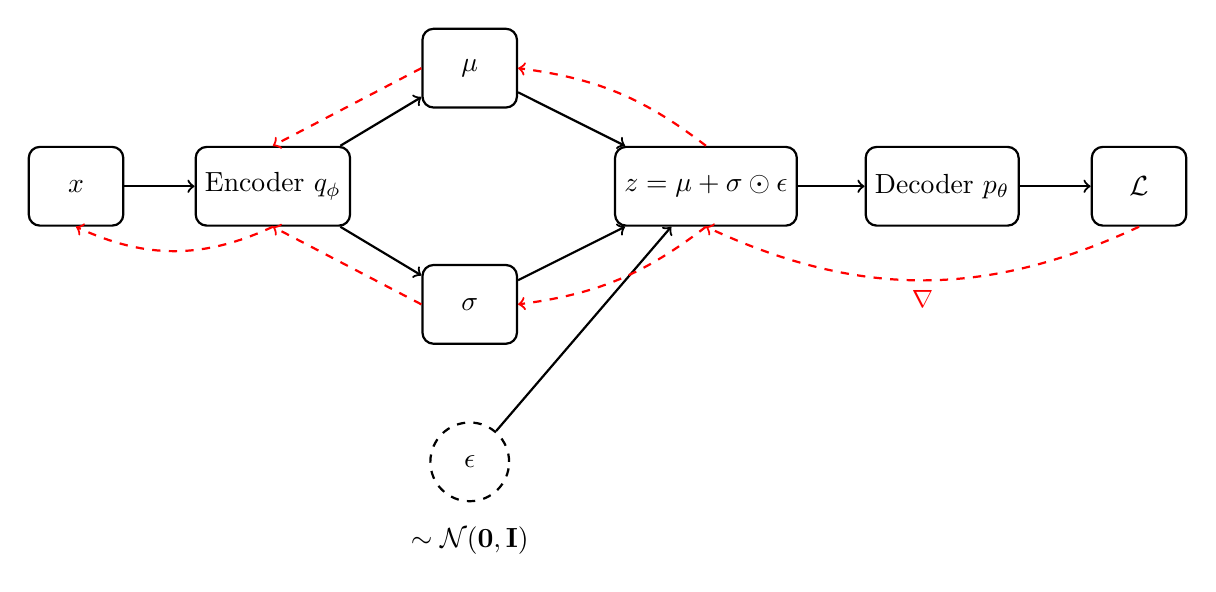
\begin{tikzpicture}[
        det/.style={rectangle, draw, rounded corners, minimum height=1cm, minimum width=1.2cm, thick},
        stoch/.style={circle, draw, dashed, minimum size=1cm, thick},
        arrow/.style={->, thick},
        grad/.style={->, thick, red, dashed}
    ]
    
    \node[det] (x) at (0,0) {$x$};
    \node[det] (enc) at (2.5,0) {Encoder $q_\phi$};
    \node[det] (mu) at (5,1.5) {$\mu$};
    \node[det] (sigma) at (5,-1.5) {$\sigma$};
    \node[stoch] (epsilon) at (5,-3.5) {$\epsilon$};
    \node[det] (z) at (8,0) {$z = \mu + \sigma \odot \epsilon$};
    \node[det] (dec) at (11,0) {Decoder $p_\theta$};
    \node[det] (loss) at (13.5,0) {$\mathcal{L}$};
    
    \draw[arrow] (x) -- (enc);
    \draw[arrow] (enc) -- (mu);
    \draw[arrow] (enc) -- (sigma);
    \draw[arrow] (mu) -- (z);
    \draw[arrow] (sigma) -- (z);
    \draw[arrow] (epsilon) -- (z);
    \draw[arrow] (z) -- (dec);
    \draw[arrow] (dec) -- (loss);
    
    % Backprop path
    \draw[grad] (loss.south) to[bend left=25] node[below] {\small $\nabla$} (z.south);
    \draw[grad] (z.north) to[bend right=15] (mu.east);
    \draw[grad] (z.south) to[bend left=15] (sigma.east);
    \draw[grad] (mu.west) -- (enc.north);
    \draw[grad] (sigma.west) -- (enc.south);
    \draw[grad] (enc.south) to[bend left=25] (x.south);
    
    \node[below] at (5,-4.2) {$\sim \mathcal{N}(\mathbf{0}, \mathbf{I})$};
    \end{tikzpicture}
    \caption{The Reparameterization Trick computational graph. Solid black arrows denote the forward evaluation pass. Dashed red arrows demonstrate the backpropagation gradients, entirely bypassing the stochastic noise node $\epsilon$.}
    \label{fig:reparam_trick}
\end{figure}

\subsection{Numerical Example: Gaussian Latent Space}
In modern implementations, the prior is overwhelmingly selected to be a standard isotropic multivariate Gaussian, $p_\theta(z) = \mathcal{N}(\mathbf{0}, \mathbf{I})$. The approximate posterior is mathematically enforced to be a multivariate Gaussian with a diagonal covariance matrix, $q_\phi(z|x) = \mathcal{N}(\mu, \text{diag}(\sigma^2))$, where both vectors are outputs of the neural network encoder.

The Kullback-Leibler divergence for a latent space of dimensionality $K$ under these conditions has a closed-form analytical solution:
\begin{equation}
    D_{\text{KL}}(\mathcal{N}(\mu, \text{diag}(\sigma^2)) \parallel \mathcal{N}(\mathbf{0}, \mathbf{I})) = \frac{1}{2} \sum_{k=1}^K \left( \sigma_k^2 + \mu_k^2 - 1 - \log(\sigma_k^2) \right)
\end{equation}

Let us step through a concrete numerical calculation. Suppose we are dealing with a $K=1$ dimensional latent space. Given a specific input $x_i$, our neural network encoder yields $\mu = 1.5$ and $\log(\sigma^2) = -0.5$.
This implies the variance is $\sigma^2 = \exp(-0.5) \approx 0.6065$, giving a standard deviation of $\sigma \approx 0.7788$.

We sample a standard normal noise variable $\epsilon \sim \mathcal{N}(0, 1)$. Suppose our random number generator provides $\epsilon = 0.8$. By Theorem \ref{thm:reparam}, the latent embedding is constructed as:
\begin{equation}
    z = \mu + \sigma \cdot \epsilon = 1.5 + 0.7788 \cdot 0.8 = 2.1230
\end{equation}
This scalar $z$ is then propagated to the decoder. Concurrently, the exact analytical KL divergence penalty acting on the parameters for this data point is computed as:
\begin{align}
    D_{\text{KL}} &= \frac{1}{2} \left( 0.6065 + (1.5)^2 - 1 - (-0.5) \right) \\
    &= \frac{1}{2} \left( 0.6065 + 2.25 - 1 + 0.5 \right) \\
    &= \frac{1}{2} \left( 2.3565 \right) = 1.17825
\end{align}
During the optimization phase, the KL gradient applies an elastic pull on $\mu$ towards $0$, and an elastic pull on $\log(\sigma^2)$ towards $0$ (yielding $\sigma^2 \to 1$). In competition, the reconstruction loss backpropagates through the sampled $z$, forcing $\mu$ and $\sigma$ to embed localized information unique to $x_i$, thereby achieving a delicate information-theoretic equilibrium.

\section{Horizon}
\begin{horizon}
The mathematical elegance of the AEVB framework assures us that we are deterministically maximizing a lower bound on the true data likelihood. Nonetheless, a substantial open problem remains regarding the ``amortization gap.'' It is conjectured that restricting inference to a feedforward network universally compromises the tightness of the ELBO compared to sample-specific iterative optimization strategies, such as Stochastic Gradient Langevin Dynamics. Future work might demonstrate that hybrid networks, combining feedforward predictions with iterative refinement steps in the latent space, can optimally close this gap without sacrificing inference speed.

Furthermore, a pervasive characteristic of the standard VAE is the blurriness of its generated samples. An intense debate remains open: is this blurriness an artifact of minimizing the expected $L_2$ norm (which rigidly assumes an isotropic Gaussian decoder likelihood), or does it arise intrinsically from the topological necessity of mapping a complex, disconnected data manifold into a dense, unimodal Gaussian prior? It is conjectured that integrating Normalizing Flows could fully close the ELBO gap, yet it remains an open question what such highly entangled prior flexibility would cost us concerning representation disentanglement.

Lastly, while AEVB seamlessly addresses continuous variables, porting these exact, unbiased, and low-variance gradient estimators to discrete categorical latent variables without resorting to biased soft-relaxations (like the Gumbel-Softmax) is a critical active frontier. We hypothesize that emerging discoveries in discrete variational bounds will eventually integrate AEVB into a sweeping, unified theory of discrete-continuous latent inference.
\end{horizon}

\section{Summary and Exercises}
\subsection{Summary}
In this chapter, we confronted the problem of intractable posterior inference within deep generative models using the Auto-Encoding Variational Bayes framework. By casting inference as a strict optimization problem, we bounded the log marginal likelihood with the Evidence Lower Bound (ELBO). To remedy the disastrous variance of gradients concerning the variational parameters, we proved the reparameterization trick, allowing gradients to deterministically flow backward through continuous random variables. 

\subsection{Exercises}
\begin{enumerate}
    \item \textbf{Analytical KL Divergence}: Prove the exact form of $D_{\text{KL}}(\mathcal{N}(\mu, \Sigma) \parallel \mathcal{N}(\mathbf{0}, \mathbf{I}))$ for a multivariate Gaussian with an arbitrary dense covariance matrix $\Sigma$. 
    \item \textbf{Variance Reduction Verification}: Consider a simple optimization of the expectation of $f(z) = z^2$. Compare the theoretical variance of the gradient estimator obtained via the standard REINFORCE (score function) algorithm to the variance of the gradient obtained via the reparameterization trick when $q(z|\phi) = \mathcal{N}(\phi, 1)$. Prove mathematically that the reparameterization trick possesses strictly lower variance.
    \item \textbf{The ELBO Gap}: Analytically prove that the discrepancy between the true log-marginal likelihood $\log p_\theta(x)$ and the ELBO $\mathcal{L}(\theta, \phi; x)$ is precisely equivalent to the Kullback-Leibler divergence between the approximate posterior and the true posterior. 
\end{enumerate}

% TODO-CITE: Ensure all named results are cited.
